\chapter{Particle Reconstruction}
\label{ch:particle_reconstruction}
	The detector does not actually measure a "particle" but merely it's presence at certain locations and energy at certain points in the detector. This information is an overwhelming mix of pixel hits, tracker hits, ECAL tower deposits, HCAL deposits, and Muon chamber hits. The raw data is nothing more than thousands of locations, times, and energy deposits. Very sophisticated software is used to connect the dots and of the hits in the tracker into likely trajectories, cluster recordings of energy in the Calorimeters into likely deposits from a showering particle, and connect muon chamber hits into another trajectory. These various pieces of information are then sewn together to reconstruct the full trajectory and energy of particles and apply a likely identification. The following sections outline the various strategies employed to identify and reconstruct information about the particles in the detector.\\	
	
	
	\section{Charged Particle Reconstruction}
	\label{sec:charged_particle_reconstruction}
	The CMS Tracker is designed as the primary measurement device for the trajectory of charged particles. Here, they leave thousands of ``hits" in the pixels and strips to mark their passage. Sophisticated algorithms use an iterative pattern recognition to assemble tracks starting from the center of the tracker. A charged particle moves in a helical trajectory (curved in the XY-plane and straight in the Z-axis). A helix is described by 5 parameters and as such the tracking algorithm starts with a very crude estimate of the parameters and searches for further hits that could match a track with those parameters, and does this layer by layer~\cite{pixel, mangano, trackingperformance}.\\
	
	There are a few variations on the tracking algorithm designed to help identify a few fringe cases, but the primary one which identifies the majority of the tracks is as follows. Hits in the inner most layers are clustered together into what is known as a ``seed." A seed has enough data (usually three hits, but some seeds with two hits are used) so that it can give a starting estimate of a particles trajectory and an error on that trajectory. The beam collision spot is also used to help determine the particle's trajectory from the seed. The seed is then used as the starting point for a combinatorial Kalman filter~\cite{ckf} which takes the trajectory estimate form the seed and looks to the next layer for a hit within a certain window of error. If it finds a hit that is consistent, then it creates a track candidate of the seed plus hit, refines he trajectory estimate and associated error, and then attempts to find a hit at the next layer. The algorithm can be tailored to look for different particles. For example a muon does not interact very much with the detector and therefore travels on a smooth trajectory. Thus muons could be searched for with a smaller window. On the other hand, an electron scatters a lot and radiates photons and therefore does not follow a very smooth trajectory. Instead it has a certain amount of random (and somewhat well quantified) random motion that can be accounted for by strategically enlarging the window to a proper size. The algorithm also employs other tricks that are often particle specific to account for multiple scattering and energy loss within the detector.\\
	
	If a hit is not found in one layer, the filter will widen the window and jump to the next layer. Although eventually tracks may be built up missing some hits in various layers, these are generally not seen as high enough quality to be used for identifying leptons, but they are occasionally still useful for something and thus are kept. Another possibility is that more than one hit may be found that falls within the window. At this point the algorithm ``branches" the track candidate into two track candidates, one containing each potential hit. In the end the one with the most total hits and the best final fit on the trajectory is kept. When tracks candidates overlap, only one is kept in the final track collection.\\
	
	Once the initial track candidates are found, they are fit with a helix. The best candidates are kept where best usually requires very few missing hits and a low error on the fit. The hits in these tracks are removed from the hit collection, and the other variations on the tracking algorithm pick through the remaining hits to find more tracks. These tracks are less likely to be as high quality as the initial group, but they are still useful and can often help in determining a charged particle's identity.\\
	
	Seeding is also performed several times using different algorithms to determine the seeds. Seeds are basically collections of two or three hits. Most of the time they are in the inner two or three layers of the tracker, but some seed algorithms that are used later will also use the two or three outer layers. There are seven seeding steps with the ones applied earliest most likely to lead to a true particle track reconstruction. The first two steps use a hit triplet from the inner layers with the most stringent seed also containing a minimum \pt cut on the particles momentum. The second one drops the \pt cut. The third step uses a hit doublet in the inner layers for additional efficiency. The fourth step is similar to the first step however it lowers the compatibility of the hits with the interaction point in order to search for tracks with displace vertices and or tracks that came from particles with longer lifetimes. The fifth step requires three hits again, but allows for them to be comprised of hits from both the pixels and the strips to allow for seeding of particles with a missed pixel hit or longer decay lengths. That last steps use pairs and triplets of hits on layers farther away from the center of the detector to find tracks of particles with a large displacement from the interaction point.\\
	
	After each step in the seeds have been propagated through the Kalman filter and associate propagation algorithms, the track candidates are fit for a final trajectory. Hits that fall too far from this trajectory are removed from the track. The five track parameters and associated errors are pulled from the final fit. Quality of the track is determined by things like vertex compatibility, number of hits in the track, and the $\chi ^2$ of the fit. As stated before, hits from tracks that are of a high enough quality are removed before the next step begins. In the end, all identified tracks from the seven steps are merged into one collection and for any tracks that overlap for a high enough number only the best candidate is kept.\\
	
		
	\section{Vertex Reconstruction}
	When an event passes a trigger, that usually means that there is some high \pt particle present in the event. This particle came from the interaction of two protons. However, for every proton-proton collision that produces an interesting particle, there are tens more in the same bunch crossing of protons that produced low energy particles that are not interesting. Particle reconstruction and measurement relies very heavily on knowing the location of the collision vertex and thus a good method for differentiation this must be used. Some examples of how knowing the accurate location of the vertex can help are: understanding the lepton impact parameter to reject muons that came from semi-leptonic decease (and thus will have a displaced vertex from the collision vertex), or identifying electrons that came from photon conversions.\\
	
	To find the vertices of the bunch crossing, first, tracks are clustered using a deterministic annealing algorithm~\cite{davtx, dacms}. Deterministic annealing algorithms have a high clustering efficiency in noisy environments like the LHC, with a vertex efficiency with a linear response function to the number of interactions. The algorithm is another iterative algorithm that clusters tracks with nearby impact parameters. It starts with large windows for the proximity of the impact parameters and tightens the window for each iteration until a stop condition is met. If a track has a transverse impact parameter \gt 3 cm or a longitudinal impact parameter \gt 4 cm it is not used in the clustering.\\
	
	Next, each cluster of tracks is used to fit a vertex position for the tracks using an adaptive vertex fitting algorithm~\cite{vertexing,vtxfit}. Tracks in the cluster that are more compatible with a vertex position for the cluster are weighted more heavily which gives a good vertex resolution of less than 50 $\mu$m (with variations in accuracy depending on the number of present tracks).\\ 
	
	
	\section{Electron Reconstruction}
	Electrons are produced in a variety of ways, but primarily the decays of interest are from bosons. This produces isolated electrons, meaning they are spatially separated from other particles in the detector. This helps in electron reconstruction, but other electron characteristics make identifying the electron harder. Electrons multiply scatter more than other particles in the tracker, radiate photons via bremstrahlung, and generally interact electromagnetically with the material they pass through. This leads to several challenges in reconstruction, on of which is a highly spread out energy distribution in the detector (both radially and angular). The main source of energy measurement for electrons is the energy deposited in the ECAL. However, this also becomes tricky to disentangle the electron energy from other deposits such as those from $\pi ^0$ which decay to photons or other hadronic particles which still start to shower in the ECAL. Thus electron identification has a goal of not only reconstructing electrons and their energy accurately, but also attempting to decide which ones originated from the proton interaction (such as electrons from boson decay) and which ones were produced later on. Details on the reconstruction of electrons, their trajectory, and their energy are discussed below while details of identifying electrons specifically from boson decay are discussed in Sec~\ref{sec:ElectronSelections}.\\
	
	Electron reconstruction is a complicated procedure and a great deal of details beyond the summary provided here may be found in~\cite{baffiReco,egmReco,egm2013}. The naive picture of an electron in the detector is a particle that leaves a track in the tracker (because is charged), leaves a large cluster of energy in the ECAL (because it interacts electromagnetically), and leaves no energy in the HCAL (because the ECAL was designed to contain any electron attempting to pass through). Thus the first piece of information to use for electron identification is a large energy deposit in the ECAL. The electron energy footprint (spacial distribution of recorded energy in the crystals) is unique. As the electron travels in the tracker its trajectory is curved in $\phi$ by the magnetic field. Due to the curved path, the general high energy of the electron, and the interactions with the tracker material, the electron will eject photons via bremstrahlung and lose energy. The photons are neutrally charged and do not curve in the magnetic field and thus encounter the ECAL spatially separate from the electron in $\phi$. Thus the total energy for the electron in the crystals once properly clustered is narrow in $\eta$ and long in $\phi$ as the photons create a long tail behind the electron. The crystals that are clustered together are called a ``Super Cluster."\\
	
	After all electron shaped SCs are assemble, they must be matched to a track in the tracker. The energy-weighted center of the SC is determined and matched to hits in the pixel detector to allow for positive charge or negative charge hypothesis. These hits are used as a seed which is then propagated out to the SC energy in a method similar to that described in  Sec~\ref{sec:charged_particle_reconstruction}. Instead of using a Kalmin filter, however, a Gaussian sum filter~\cite{gsf} is used to better account for the erratic path of an electron that interacts with the tracker and changes trajectory through bremstrahlung.\\
	
	For some difficult problems like electron reconstruction. CMS uses two different methods to and merges the results. In this case, a second method is employed using Particle-Flow (PF) based algorithms. PF algorithms will be described in more detail in Sec~\ref{sec:pf_algorithm}. Essentially, PF electron reconstruction starts in the tracker and ``swims" outward connecting hits into tracks and then connecting tracks to energy deposits in the ECAl and the HCAL. At each step in the track building, the algorithm uses the current best trajectory guess to search for compatible ECAL clusters that originate from a radiated photon. In this way it builds a detailed map of all of the particles and doesn't just lump them all into a single particle (although the energy of the radiated photon is counted as part of the electron's energy).\\
	
	After both algorithms have run, the collections of electrons are merged. At electron energies \gt 20 \GeV, the SC seeded algorithm is responsible for the majority of the reconstruction while at energies below this, the PF method demonstrates much better efficiency. The PF method also does better in crowded environments (non-isolated electrons) due to it's ability to differentiate sources of energy better because it tracks individual components of a shower. See Fig~\ref{fig:electron_reconstruction} for an illustration of the electrons built by the two methods.\\
	
	
		\begin{figure}[h]
\begin{center}
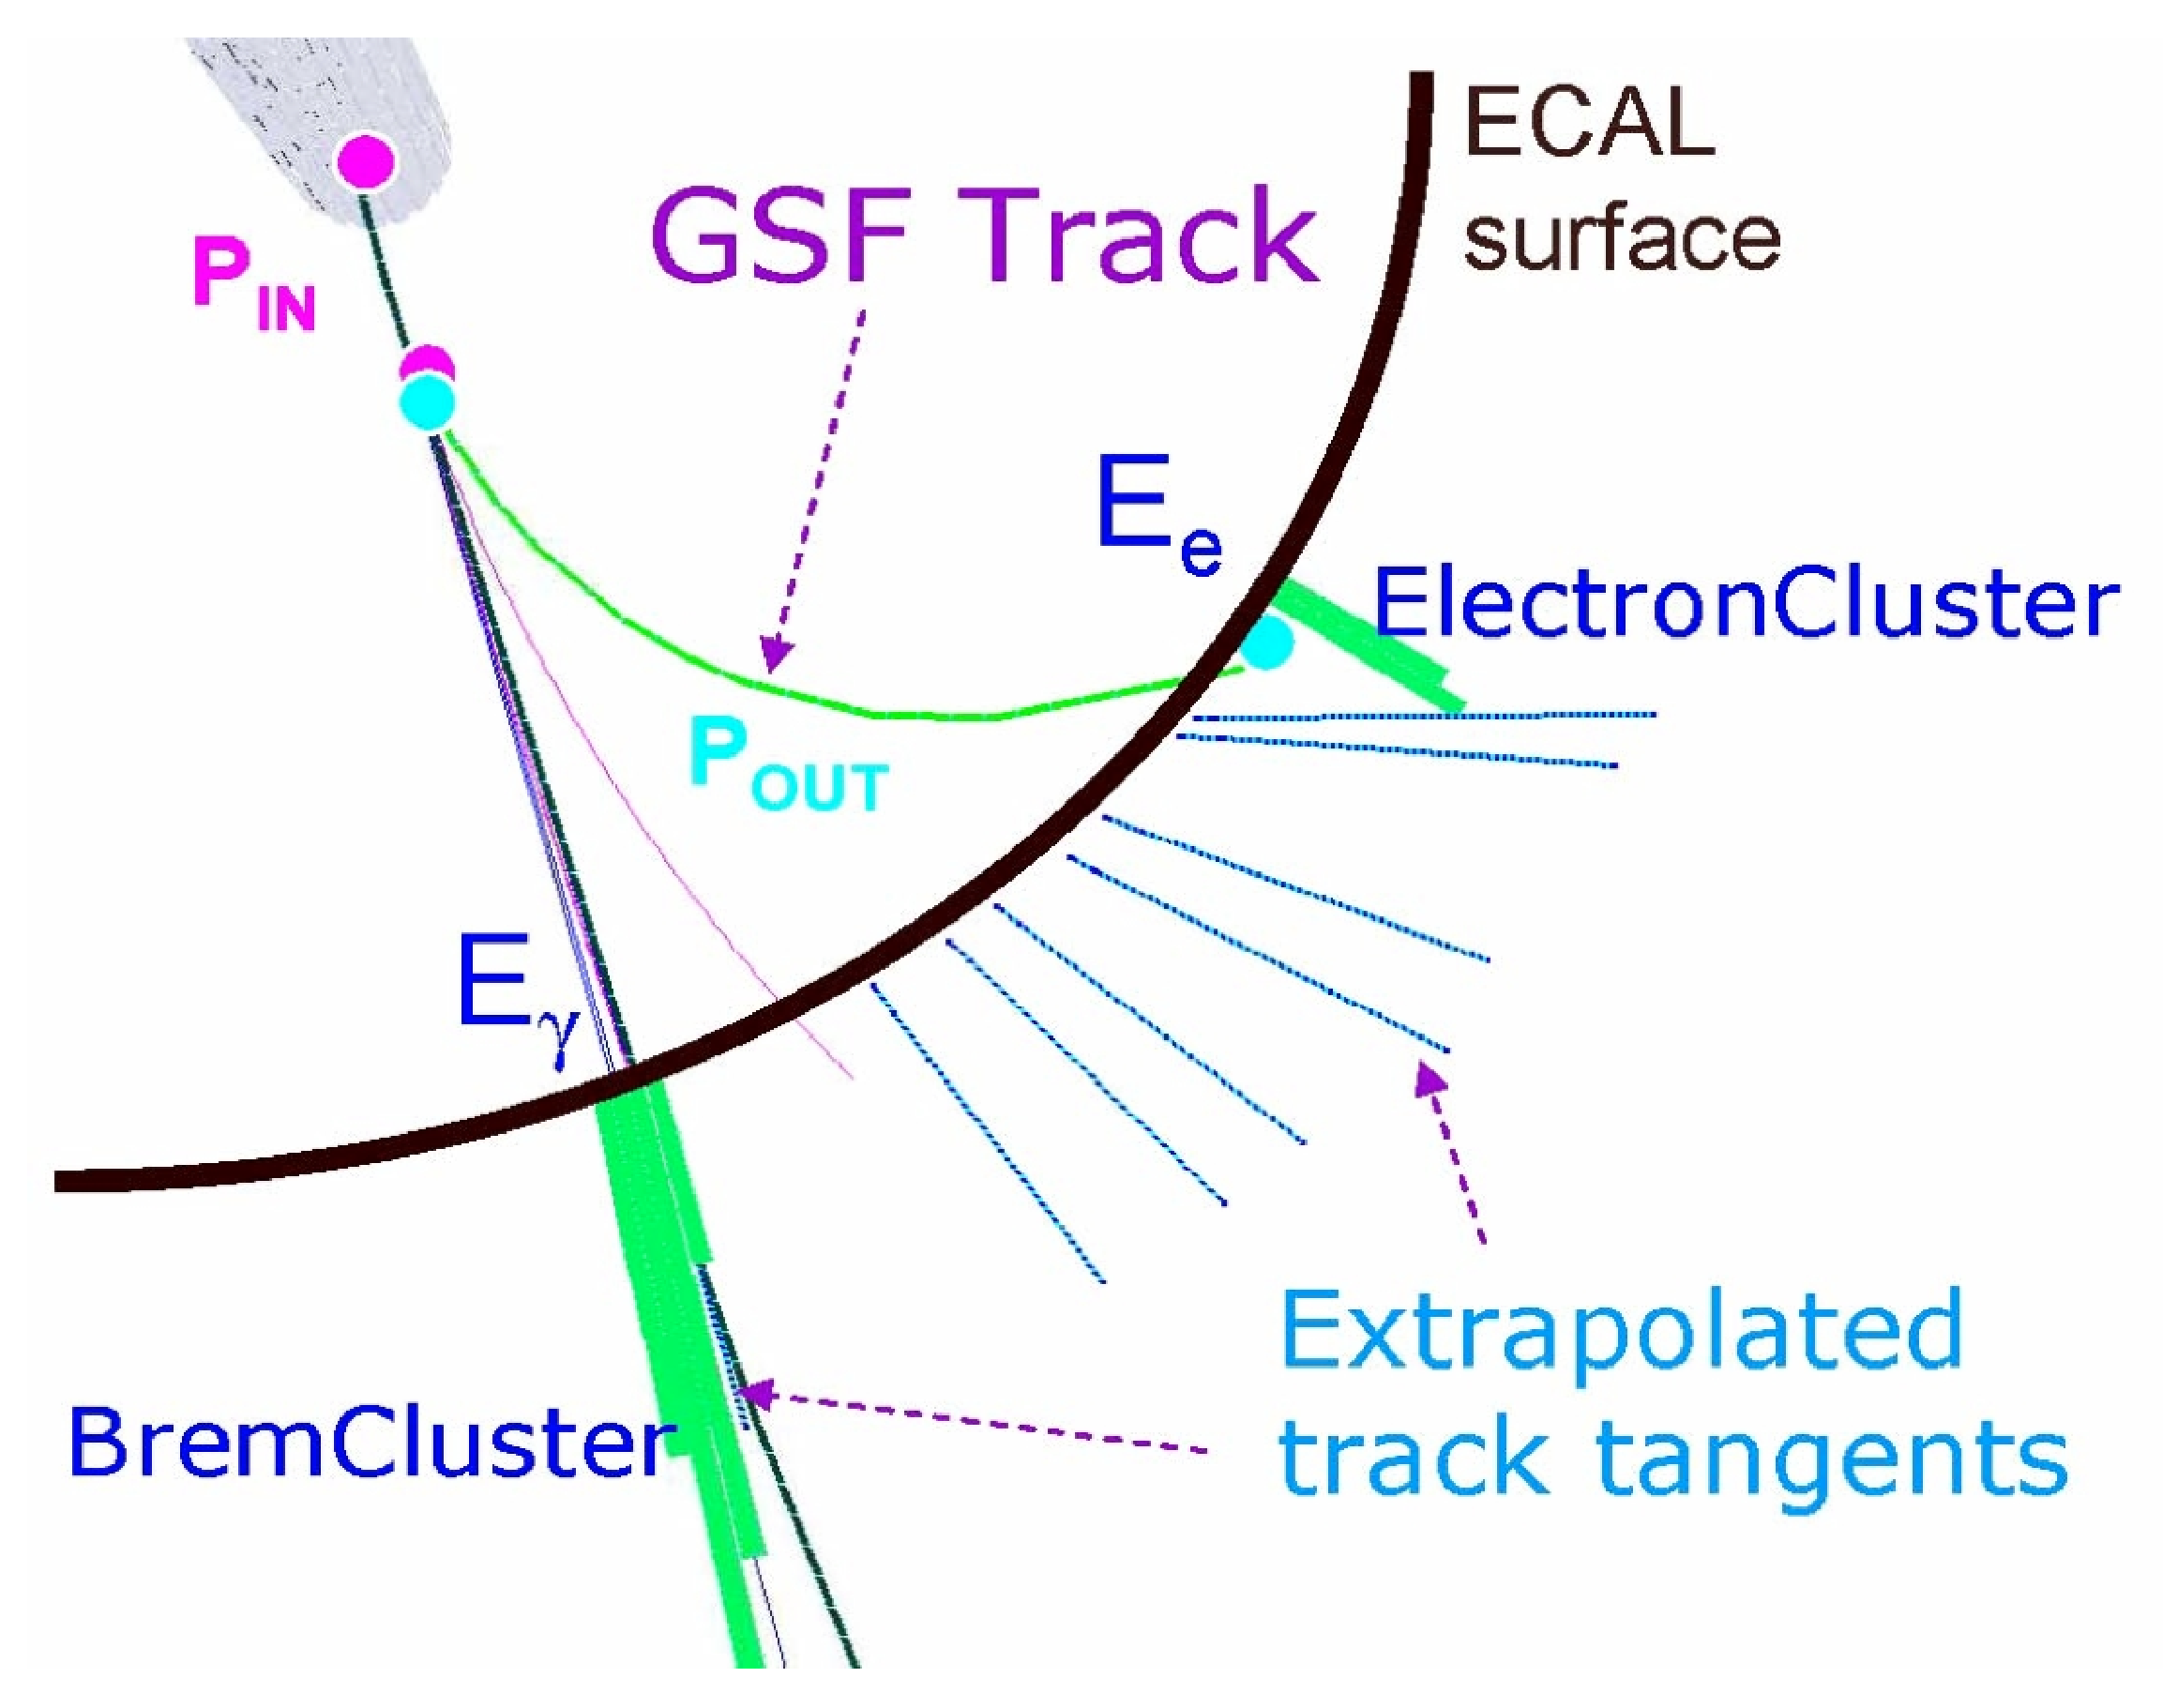
\includegraphics[width=0.70\linewidth]{Figs/elereco.pdf}
\caption{\label{fig:electron_reconstruction}
Graphical representation of the stages of an electron in the detector and the components that must be combined in the reconstruction. The electron bremsstrahlungs a photon which leaves a region of energy in the ECAL. The electron itself leaves energy in the ECAL near the photon's energy along a somewhat predictable curved trajectory~\cite{bourge}.
}
\end{center}
\end{figure}
	
	
	
	
	
	
	\section{Muon Reconstruction}
	Muons do not suffer from many of the challenges of electrons. At the energies in the LHC, they do not radiate photons or interact with the material in the detector. They follow fairly straight forward trajectories and leave tracks in the muon chamber but no energy in either of the calorimeters. Identification involves using both the tracks in the tracker and hits in the muon chamber which create two trajectories that match up (but curve in opposite directions due to the change in magnetic field direction outside the calorimeters). Therefore, muon reconstruction efficiency is quite high. Sometimes pions that travel farther through the HCAL than they statistically should ``punch through" into the muon chamber to be reconstructed as muons. These pions and muons from semi-leptonic decays are the main sources of ``muons" which do not come the primary interaction point (e.g. boson decays). Algorithms for removing false positives are discussed in Sec~\ref{sec:MuonSelections}. Muon reconstruction algorithms are discussed in detail in these References~\cite{muontdr,muonReco}.\\
	
	Due to the blocking power of he calorimeters and the iron return yolk, the logical place to start a muon reconstruction algorithm is in the muon chamber where very few particles from the collision reach. DT and CSC hits are matched together to form small track like segments compatible with a single particle's trajectory. Then RPC measurements are used to for additional position measurements. Tracking begins from the inside of the muon system to the outside using a Kalmin filter that accounts for energy loss as the muon travels through the many iron layers. Tracks fit in the just the muon system are known as ``Stand Alone Muons" (SA Muons).\\
	
	The SA muons are then used to pick out compatible tracks in the tracker matching opposite curvature, energy, and trajectory. All of the positional hits from both the track and the SA muon are used again for a refit. At this point, some of the tacker hits or muon system hits may be dropped if they don't work in the overall fit (even if they did work in one of the individual parts) so that the ``Global" muon is not merely the track and SA muon added together.\\
	
	A third method is employed that starts in the tracker. It starts by using a track in an analogous way to a seed (from track building) and uses expected trajectory and uncertainty from material interaction to find segments in the muon chamber starting from the inside out. The total energy in the ECAL and HCAL at the expected crossing is checked to ensure that it is small enough to be compatible with the passing of a minimum ionizing particle. By building a muon track from the tracker out, these ``Tracker" muons may not completely match either SA or Global muons. In fact Tracker muons have a higher reconstruction efficiency for low \pt muons, but have a draw back of allowing more ``fake" muons to be reconstructed.  SA, Global, and Tracker muons may be combined (for example asking if they share a certain fraction of hits) to ensure even higher quality muons as well as other selections applied to reduce the false positive backgrounds.\\
	
	
	
			\begin{figure}[h]
\begin{center}

\includegraphics[width=0.48\linewidth]{Figs/placeholder.pdf}
\caption{\label{fig:muon_reconstruction}
.
}
\end{center}
\end{figure}
	
	
	
	
	\section{Particle Flow Candidate Reconstruction}
	\label{sec:pf_algorithm}
	
	During the early runs of CMS, a new method for reconstructing particles was implemented. This method shifts from a detector component based method of identifying and reconstructing particles, their energy/momentum, and trajectory by piecing together the information from the sub-detectors to a more holistic method that uses all of the sub-detectors at once. This method is known as the ``Particle Flow" (PF) algorithm. The PF algorithm attempts to identify the path of all the particles through the detector so that a complete list can be assembled.\\
	
	Detector based methods have been used in other experiments and are still used to varying degrees in CMS. One reason to shift towards PF based methods is that Detector based methods have the potential to double count energy deposits whereas PF methods do not suffer from this as they do a global reconstruction particle by particle. At this point, PF based methods are the primary and collaboration recommended methods for the calculation of missing transverse energy (\met), jet reconstruction, and 
$\tau$ reconstruction. For more details on the PF method than are provided here, see References~\cite{pfReco,pfComm}.\\

	In the PF algorithm, local reconstructions are performed in the sub-detectors in ways similar to what has been previously described for Detector based reconstruction. However, at this point, objects from each sub detector that are near to each other are grouped together into blocks. Blocks will usually contain inputs from at least 2 different sub-detectors (For example energy in the ECAL and HCAL or a track pointing towards large amounts of energy in the HCAL). At this point the general strategy is to then link the blocks together in a meaningful way. Blocks that can be linked together to form compatible electron or muon signatures are removed from the set first and place in the PF collection as electrons and muons. Additionally, any clusters that can be linked to radiated products from these particles are removed and placed in the PF list (e.g. photons linked to an electron). Electrons and muons are chosen first because they have very clean signatures when they are decay products of bosons and thus have a higher efficiency for reconstruction. The second round attempts to identify hadrons by comparing track momentum to connected ECAL and HCAL energy. If the energy and momentum are compatible then this object is placed in the PF charged hadron collection and its energy is estimated as a weighted sum of both objects. The blocks of this charged hadron are removed from the list and other linked constituents from showering are also removed from the list and added to the PF charged hadron list. However, this could be a muon, and so a test is performed to see if the momentum has significantly more momentum than is compatible with the energy deposited in the calorimeters. In this case a secondary muon identification algorithm is performed that is optimized for non-isolated lower \pt muons and successful matches are placed in the muon list. Should significantly more energy be found in the calorimeters, then neutral hadrons and photons are reconstructed using the excess energy in the calorimeters that are not accounted for with the matched track. Finally, any remaining unlinked ECAL clusters are assumed to be photons and all remaining unlinked HCAL clusters are assumed to be neutral hadrons. Both are added to the respective lists.\\
	
	
	
	
	
	\section{Jets Reconstruction}
	Hadron colliders produce physical scenarios where the constituents of hadrons collide. At the LHC, the collisions are between the quarks and gluons inside the protons. This leads to production scenarios with a lot of particles with color charge. Spare gluons often accompany events. Bosons often decay to quarks. Tops decay to b-quarks. And so on. Due to color confinement and the nature of the strong force, quarks do not exist on their own for very long and go through a showering process known as hadronization where quark/anti-quark pairs are pulled out of the vacuum to attempt to produce a color neutral object. The particles fly in roughly the same direction and continue showering in a cone-like formation. All of these particles leave some energy in the ECAL and a lot of energy in the HCAL. This collimated spray of energy is known as a ``jet." Gluons similarly produce jets. Gluons can be radiated off of quarks before or after a collision and the gluons decay 100\% to quarks which shower as one or more jets. Thus jet reconstruction is a bit messy as it must recombine a number of particles and energy deposits into one origin and composite particle.\\
	
	The current best method of jet reconstruction relies on PF candidates (see Sec~\ref{sec:pf_algorithm}) which attempt to track individual particles through the detector. Nearby charged and neutral hadronic candidates are clustered together. The highest \pt PF candidates are assumed to be somewhat central in a jet and are thus used as the clustering seed. Candidates are clustered using the anti-$k_T$ algorithm~\cite{antikt} with a distance parameter of $\Delta R$ = 0.5, where $\Delta R$ is defined in the $\eta - \phi$ plain. The anti-$k_T$ algorithm uses a distance measurement that is inversely proportional to the square of each candidate's \pt. Those who do theoretical work on jets recommend the anti-$k_T$ algorithm because it provides safety against infrared and collinear radiation, unlike other methods with can fail under these conditions. This allows the theorists to work on advancing the theoretical knowledge of how jets behave in experimental settings.\\
	
	Jet reconstruction with detector based methods suffered from poor response function and energy reconstruction efficiency. To compensate, detector based jets used several levels of correction to account for the average error in energy reconstruction based on monument and direction of the jets. Reconstruction based on the PF method is better due to the PF algorithms handling of individual particles (charged hadrons and photons especially which make up 90\% of the showering jet) and it's ability to link them together to a common source. Some corrections are still applied to PF based jets, but by and large the results are more accurate (see~\cite{cmsjetcal}). The corrections take three steps:
	\begin{enumerate}
	\item Ambient energy from other particles in the event can seep into the PF jet's energy measurement. These other particles often come from other collisions in the same bunch crossing and are known as ``pile-up." The mean energy density of the pile-up is calculated using a FastJet~\cite{fastjet} method coupled with a ghost particle method for calculating jet areas~\cite{jetarea}. This background energy is subtracted from the PF jet.
	\item The detector does not have the same response for particles of different $\eta$ and \pt. The response function based on $\eta$ and \pt is determined in simulation and applied to the PF jet.
	\item Finally the differences between response of the CMS detector and the simulations is applied. Di-jet samples, $\gamma$+jets, and Z+jets samples are used in data and Monte Carlo simulation. In these events conservation of momentum is used to balance the products recoiling off of each other (e.g. the Z recoiling off of the jet) to more accurately measure the true energy of the jet with the objects that are better measured (e.g. a Z). This methods yields an uncertainty of \lt 5\% which is smaller than the jet energy resolution in the detector (between 8\% and 15\% depending on momentum and direction of the jet).
	\end{enumerate}
	
	Finally, for data only there is a residual correction.\\
	
	
	
	
	\section{Reconstruction of Jets from b-quarks}
	\label{sec:csv_reconstruction}
	
	For most intents and purposes jets originating from u, d, c, and s quarks are treated as the same thing at CMS. Because of their masses, b- and top-quarks behave differently and can be specifically identified. Top quarks are so massive that they don't hadronize and thus do not get measured as jets, but instead decay to a b-quark and a W boson 100\% of the time. b-quarks are massive, but do hadronize. Because events that produce top quarks are very useful in many physics searches at CMS, accurately measuring and identifying b-jets is very important as b-quarks are one of the more helpful discriminators for the presence of a top quark. Due to their mass, b-jets have a major defining feature. If the constituent hadronic particles are traced back to an origin (jet vertex), that vertex is displaced by a predictable margin from the primary interaction point (primary vertex). The lighter quarks that form other jets do not have displaced vertices. Several methods exist to identify the b-jets, but at the time of this work, the best algorithm was a Multi-Variate Analysis (MVA) based method known as the Combined Secondary Vertex method (CSV)~\cite{btagging}. Details about the use and associated errors for this method will be described in Sec~\ref{sec:btag_syst} while a brief summary of how it works is in the following.\\
	
	In this method, the b-jet vertex is known as the secondary vertex and the collision vertex is known as the primary vertex. Two pieces of information are used heavily:
	\begin{enumerate}
	\item Distance between the primary and secondary vertex. This distance should fall into a well-defined window.
	\item Direction between the primary vertex, the secondary vertex, and the b-jet. To be compatible, the two vertices follow the trajectory of the b-jet shower. If for example the primary vertex is in between the secondary vertex and the jet track, this is not a compatible jet.
	\end{enumerate}
	
	Additionally, the significance of the flight distance (ratio of flight distance to error on that distance) can be used with the distance to make that variable more discriminating. The CSV algorithm combines the flight distance information with track-based lifetime information. This algorithm also can use parts of this information when no secondary vertices are found to attempt to increase efficiency of b-jet identification. There are three vertex categories:
	\begin{itemize}
	\item Real: A secondary vertex has been identified.
	\item Pseudo: When a secondary vertex is not identified, the algorithm looks at the impact parameter significance (impact parameter divide by it's uncertainty) of the jet to define a Pseudo vertex.
	\item No Vertex: When both the above categories fail.
	\end{itemize}
	
	As an MVA based method, the CSV algorithm takes into account a number of different variables. For the real and pseudo vertex category, all of the variables are used in addition to vertex category. For the no vertex category, only the last two are used.
	\begin{itemize}
	\item Significance of the flight distance in the transverse plane (distance in x-y divided by the error of that distance).
	\item Invariant mass of particles traced back to the secondary vertex.
	\item Ratio of the energy of the tracks clustered in the jet traced back to the secondary vertex to the energy of the tracks clustered in the jet that do not trace back to the secondary vertex.
	\item The pseudorapidity of the tracks traced to the secondary vertex with respect to the pseudorapidity of the jet.
	\item The impact parameter significance in the transverse plane of the first track which causes the invariant mass of the jet to be larger than 1.5 \GeVcc (the mass of the charm quark).
	\item Total number of tracks clustered in the jet.
	\item The impact parameter significance in all three spatial directions for each track clustered in the jet.
	\end{itemize}
	
	The MVA builds a likelihood ratio from these variables which combines their values in multivariate space to produce one discriminating value. This value can be used to discriminate between b-jets and c-jets (c-jets also can behave slightly differently from u- and d-jets but at CMS, this information tends not to be used) as well as between b-jets and light flavor- (u- and d-) jets. Three working points are chosen for different levels of efficiency: Tight, Medium, and Loose, with Tight having the highest purity of b-jets and the lowest efficiency for accepting real b-jets and with Loose having the lowest purity of b-jets, but the highest efficiency for accepting b-jets. More information on how this discriminate is used can be found in Sec~\ref{sec:bTagSelection}. See Fig~\ref{fig:csv_discriminant_values} for a plot of values and composition in data and MC.
	
	
\begin{figure}[h]
\begin{center}
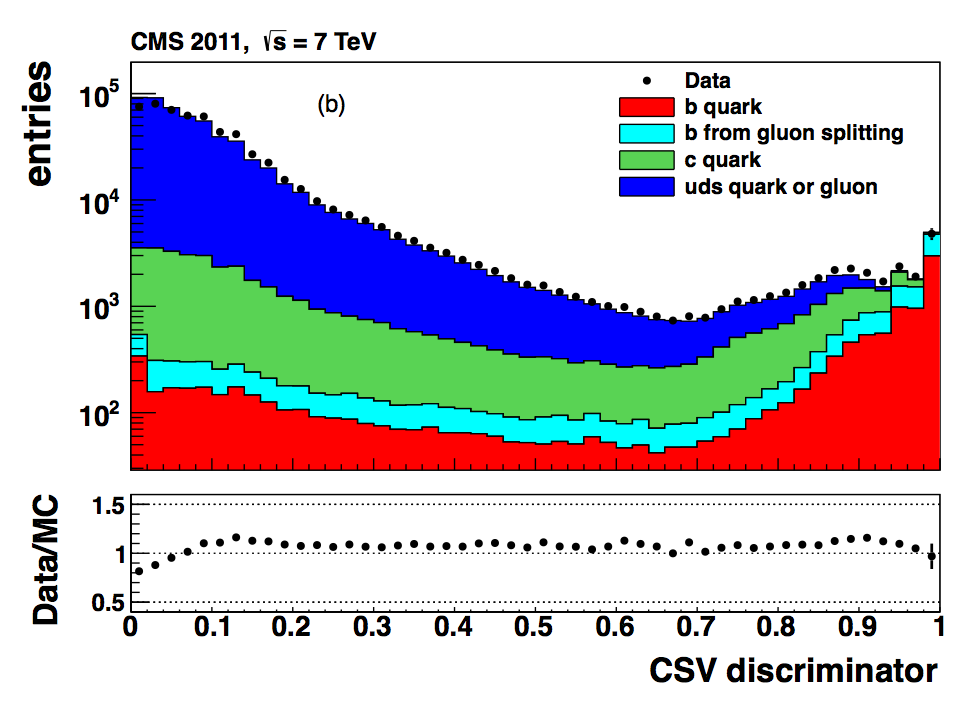
\includegraphics[width=0.7\linewidth]{Figs/CSV_discriminator_values.png}
\caption{\label{fig:csv_discriminant_values}
Plot of data and MC overlaid. The MC contains samples of jets originating from different quarks including b and light flavor~\cite{btagging}.
}
\end{center}
\end{figure}
	
	
	
	
	
	
	
	
	
	